\documentclass{beamer}

\usetheme{Singapore}

\usepackage{float}
\usepackage{multimedia}
\usepackage{color}
\usepackage{color}
\definecolor{DarkBlue}{rgb}{0.1,0.1,0.5}
\definecolor{Black}{rgb}{0,0,0}
\definecolor{Blue}{rgb}{0.1,0.1,0.9}
\definecolor{Red}{rgb}{0.9,0.0,0.1}
\definecolor{Green}{rgb}{0.0,0.9,0.0}
\definecolor{DeadGreen}{rgb}{0.3,0.6,0.3}
\definecolor{Brown}{rgb}{0.5,0.3,0.4}
\usepackage{polski}
\usepackage[utf8]{inputenc}
\usepackage{caption}
\usepackage{subcaption}

\title{Docker i Kubernetes w zarządzaniu projektem informatycznym}
\author{promotor: dr hab. Serweryn Kowalski, prof. UŚ}
\subtitle{Ewa Namysł}
\institute{Uniwersytet Śląski}
\date{22. listopada 2022}

\begin{document}

%STRONA TYTUŁOWA
\frame{
	\titlepage
}

%SPIS TREŚCI
\frame{
	\tableofcontents
	\frametitle{Spis treści}
}


\section{Maszyna fizyczna}

\frame{
	\frametitle{Postępy w pracy}
	\centering

	\textbf{Skonfigurowanie środowiska pracy na maszynie fizycznej}
	\vspace{1em}
	\begin{itemize}		
		\item System operacyjny: CentOS Stream 9
		\item Instalacja biblioteki libvirt - niezbędnej do wykorzystania Vagranta w wirtualizacji przy pomocy KVM/QEMU
		\item Instalacja pakietu Vagrant w celu tworzenia plików konfiguracyjnych dla maszyn wirtualnych
		\item Otwarcie i przekierowanie portów na maszynie fizycznej, aby umożliwić zdalny dostęp do serwisów
	\end{itemize}
}

\frame{
	\frametitle{Postępy w pracy}
	\centering

	\textbf{Diagram}
	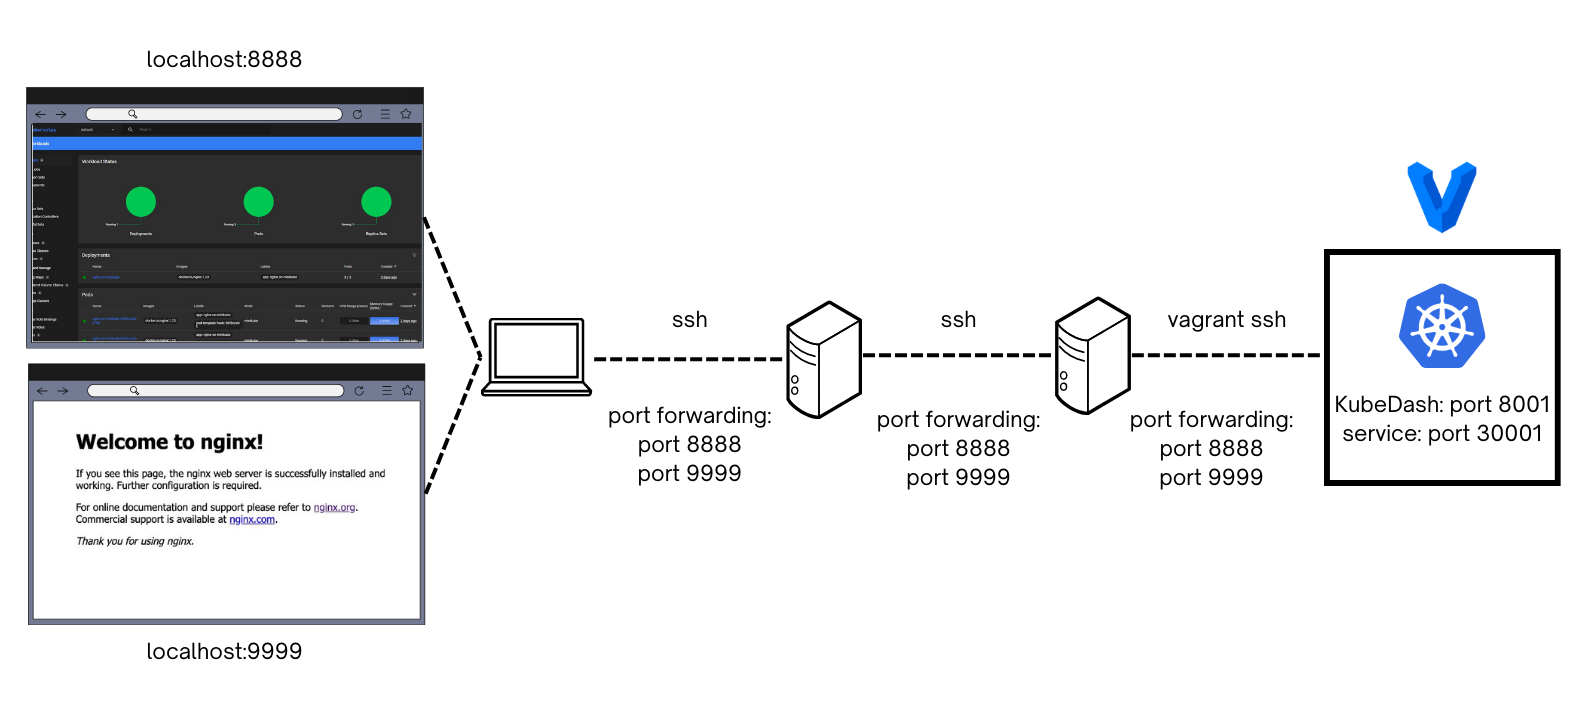
\includegraphics[scale=0.2]{diagram.png}
}

\section{Maszyna wirtualna}

\frame{
	\frametitle{Postępy w pracy}
	\centering

	\textbf{Pierwsza wersja maszyny wirtualnej}
	\vspace{1em}
	\begin{itemize}		
		\item tworzenie podstawowego pliku Vagrantfile:
	\end{itemize}

	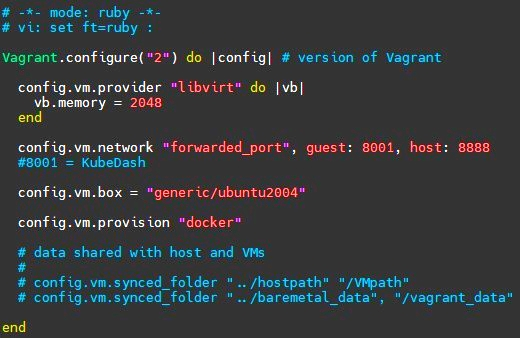
\includegraphics[scale=0.7]{vagrantfile.jpg}
}

\frame{
	\frametitle{Postępy w pracy}
	\centering

	\begin{itemize}		
		\item Dalsza automatyzacja procesu tworzenia VM:
	\end{itemize} 

	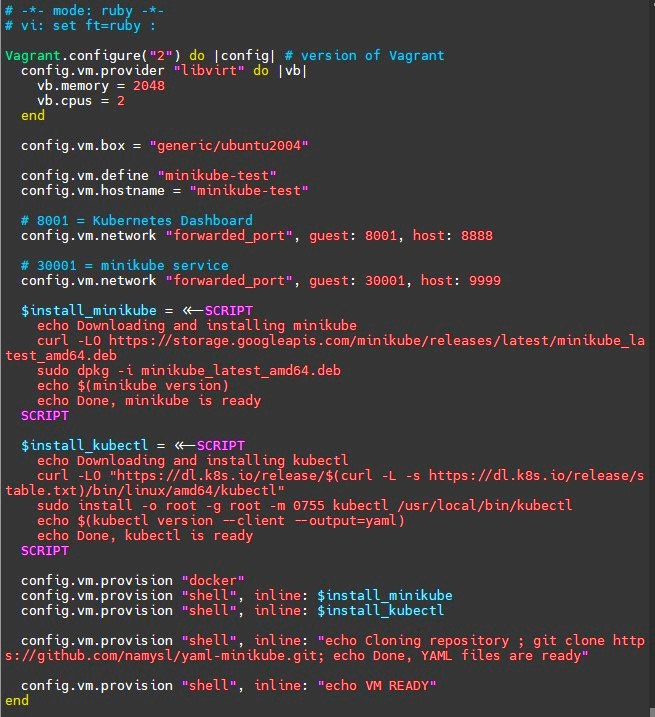
\includegraphics[scale=0.4]{vagrantfile2.jpg}
}

\frame{
	\frametitle{Postępy w pracy}
	\centering

	\textbf{Uruchamianie maszyny wirtualnej}
	\vspace{1em}
	\begin{itemize}		
		\item włączenie maszyny poprzez komendę vagrant up
		\item sprawdzenie statusu
		\item łączenie się z maszyną przez SSH
	\end{itemize}

	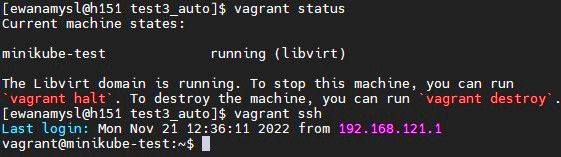
\includegraphics[scale=0.7]{vagrant2.jpg}
}

\section{Kubernetes}

\frame{
	\frametitle{Postępy w pracy}
	\centering

	\textbf{Pliki YAML}
	\vspace{1em}
	\begin{itemize}
		\item Stworzenie plików YAML dla deploymentu i service'u
		\item Hosting na GitHubie, ściąganie plików w trakcie tworzenia VM
	\end{itemize}

	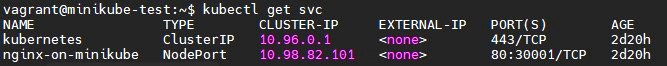
\includegraphics[scale=0.6]{svc.jpg}
}

\frame{
	\frametitle{YAML deployment}
	\centering
	kubectl apply -f yaml-minikube/deployment.yaml
	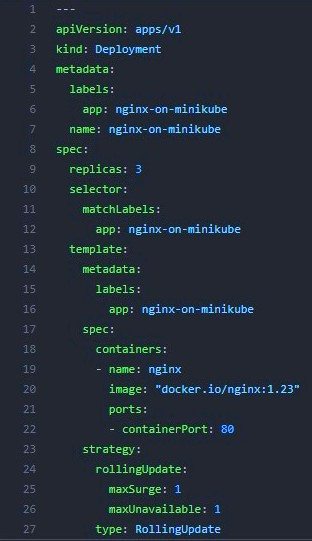
\includegraphics[scale=0.4]{depl.jpg}
}

\frame{
	\frametitle{YAML service}
	\centering
	kubectl apply -f yaml-minikube/service.yaml
	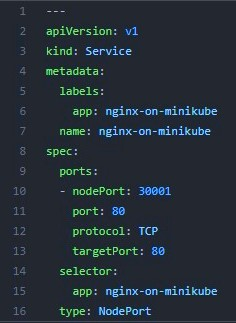
\includegraphics[scale=0.6]{serv.jpg}
}

\frame{
	\frametitle{Dostęp do Kubernetes Dashboard}
	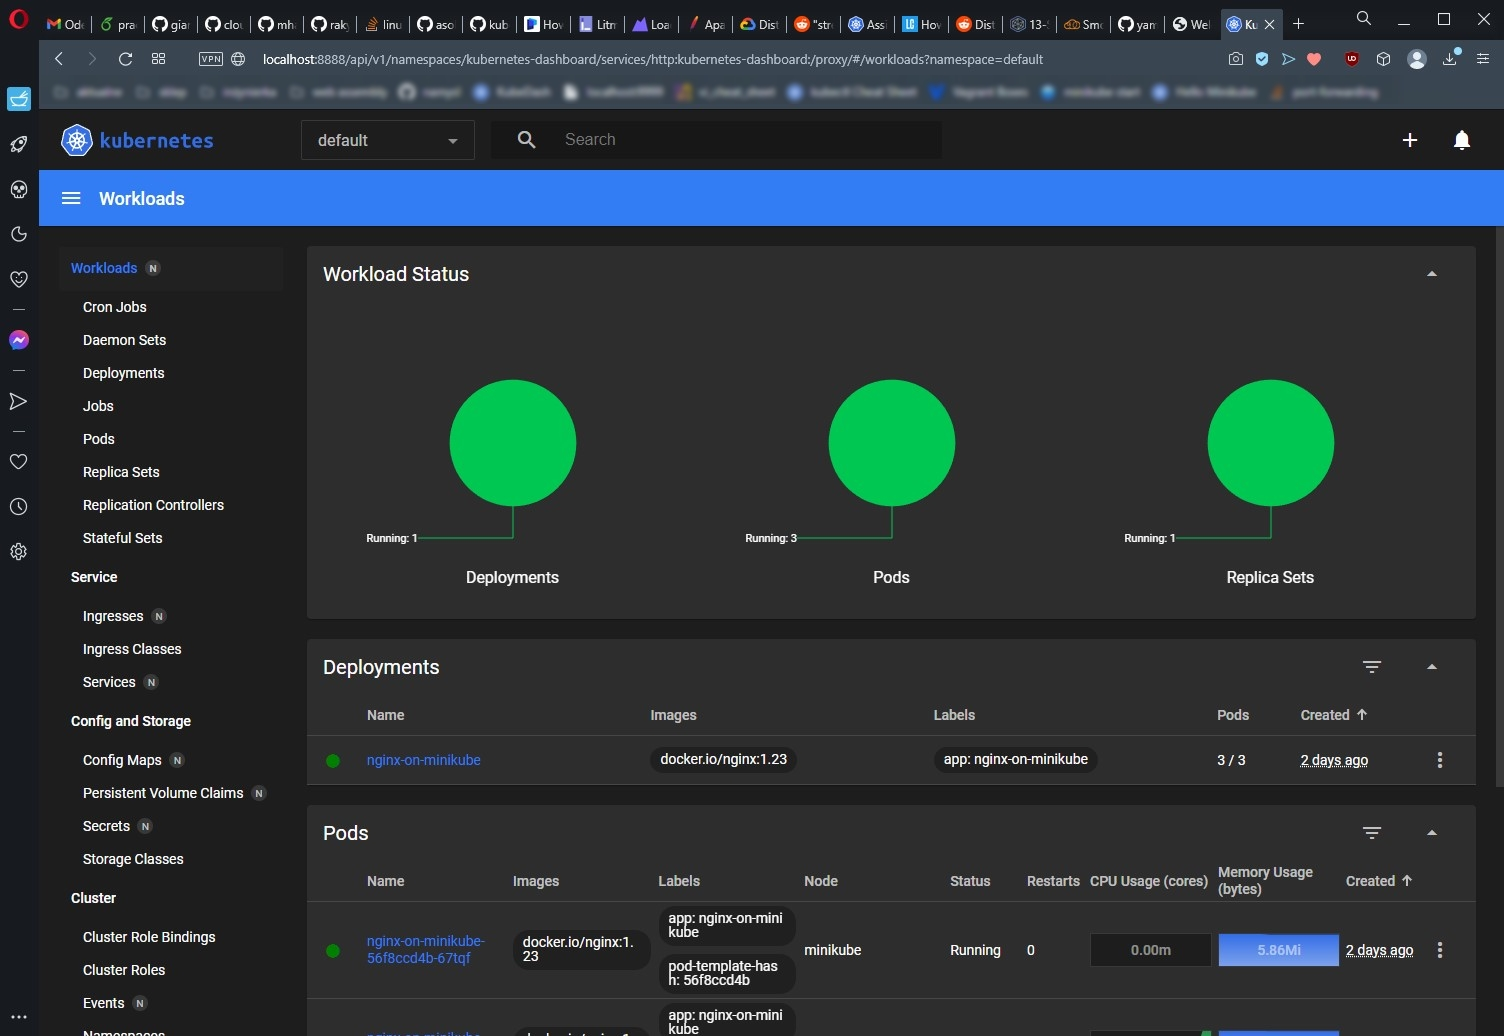
\includegraphics[scale=0.27]{kubedash.jpg}
}


\frame{
	\frametitle{Lokalne testowanie aplikacji}
	\centering
	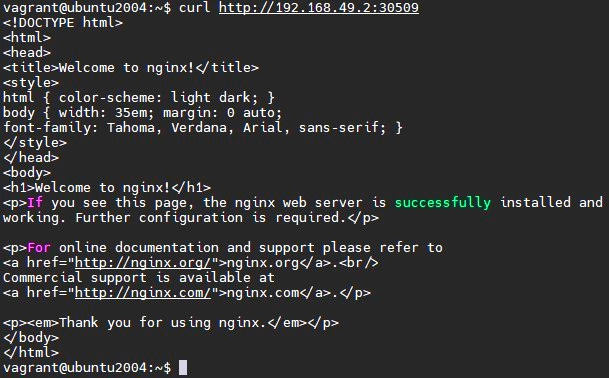
\includegraphics[scale=0.6]{curl.jpg}
}


\frame{
	\frametitle{Zdalny dostęp}
	\centering
	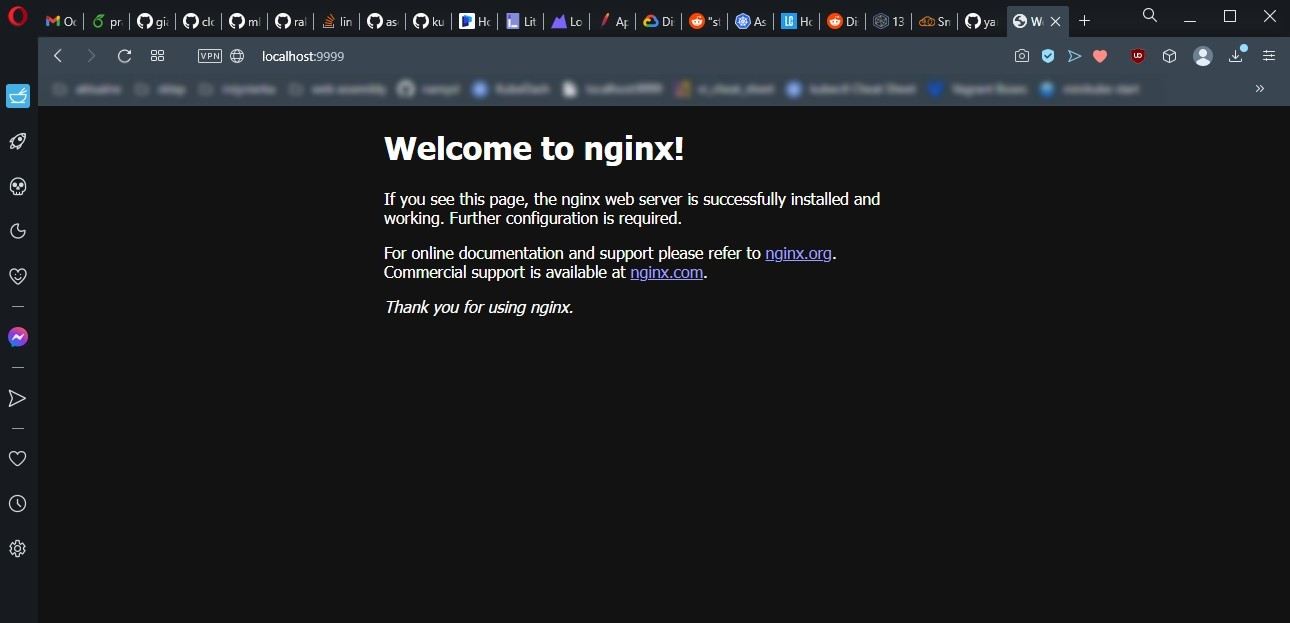
\includegraphics[scale=0.25]{localhost.jpg}
}

\frame{
	\frametitle{Postępy w pracy}
	\centering

	\textbf{Przetestowano:}
	\begin{itemize}
		\item dostęp do podów i wprowadzanie w nich zmian,
		\item rolling updates, czyli update deploymentu bez downtime'u,
		\item niszczenie podów,
		\item zbieranie i interpretowanie logów
	\end{itemize}
}


\section{Kolejny etap}
\frame{
	\frametitle{Kolejny etap}
	\centering

	\vspace{1em}
	\begin{itemize}
		\item Wprowadzenie horizontal pod autoscalera i limitu zasobów,
		\item Przeprowadzenie stress testów na minikube,
		\item Rozpoczęcie pracy nad plikiem Vagrantfile dla większej liczby węzłów (1 master, 2 workery)
	\end{itemize}
}

\frame{
	\frametitle{Bibliografia}
	\vspace{1em}
	Kubernetes - oficjalna dokumentacja. \\ https://kubernetes.io/docs/ \\Dostęp: 2022-11-05\\
	\vspace{1em}
	Vagrant - oficjalna dokumentacja. \\ https://www.vagrantup.com/docs/ \\Dostęp: 2022-11-05\\
	\vspace{1em}
	E. Nemeth, G. Snyder, T. R. Hein, B. Whaley, D. Mackin.\\ Unix i Linux.
Przewodnik administratora systemów. \\Wydawnictwo HELION, 2018. \\

}

\end{document}